% !TeX spellcheck = cs_CZ
%{\tikzset{external/prefix={tikz/FYZII/}}
% \tikzset{external/figure name/.add={ch12_}{}}
%---------------------------------------------------------------------------------------------------
% file fey2ch12.tex
%---------------------------------------------------------------------------------------------------
%=========================== Kapitola: Analogie elektrostatiky =====================================
\setchaptertoc
\chapter{Analogie elektrostatiky}\label{fyz:IIchapXII}  
  \section{Stejné rovnice mají stejné řešení}\label{fyz:IIchapXIIsecI}
    Celkové množství informací, které se od začátku vědeckého pokroku o fyzikálním světě
    nashromáždilo, je ohromné a zdá se téměř nemožné, aby si z něj jednodivec dokázal osvojit
    nějakou dostatečně rozsáhlou část. Ale ve skutečnosti si fyzik spíše dokáže uchovat široké
    vědomosti o fyzikálním světě, než se stát specialistou v nějaké úzké oblasti. Má to tři příčiny:
    Zaprvé, existují velké principy, jež platí pro všechny různé druhy jevů - například principy
    zachování energie a momentu hybnosti. Důkladné pochopení takových principů umožňuje porozumět
    mnoha věcem najednou. Za druhé, faktem je, že mnohé složité jevy, např. vlastnosti pevných těles
    pod tlakem, jsou v podstatě určeny elektrickými a kvantově mechanickými silami; porozumí-li tedy
    někdo základním zákonům elektřiny a kvantové mechaniky, vyplývá z toho přinejmenším určitá
    možnost porozumět mnoha jevům, k nimž dochází ve složitých situacích. Nakonec, existuje tato
    nejpozoruhodnější shoda: \emph{rovnice pro mnohé odlišné fyzikální problémy vypadají přesně
    stejně}. Pravda, symboly se přitom mohou lišit - jedno písmeno je nahrazeno jiným, ale
    matematický tvar rovnic je tentýž. Znamená to, že jestliže jsme prozkoumali jednu věc, okamžitě
    jsme dostali mnoho přesných poznatků i o řešení jiných problémů.

    Nyní jsme skončili s elektrostatikou a brzy budeme pokračovat studiem magnetizmu a
    elektrodynamiky. Ale ještě předtím bychom rádi ukázali, že při studiu elektrostatiky jsme se
    současně dozvěděli i o velkém počtu jiných témat. Uvidíme, že rovnice elektrostatiky se
    vyskytují i na několika jiných místech ve fyzice. Přímým přenesením jejich řešení (samozřejmě,
    stejné matematické rovnice musí mít stejná řešení) je možné řešit úlohy v jiných oblastech
    stejně snadno - nebo stejně obtížně - jako v elektrostatice.

    Jak víme, rovnice elektrostatiky vypadají takto:
    \begin{subequations}
      \begin{align}
         \nabla\cdot(\varepsilon_r\vec{E})&=\dfrac{\varrho_{vol}}{\varepsilon_0},\label{fyz:eq756}\\  
         \nabla\times\vec{E}              &= 0.                                  \label{fyz:eq757}
      \end{align}
    \end{subequations}
    (Uvádíme rovnice elektrostatiky pro dielektrika, abychom měli co nejobecnější situaci.) Tentýž
    fyzikální obsah je možno vyjádřit v jiném matematickém tvaru:
    \begin{subequations}
      \begin{align}
         \vec{E}  &=-\nabla\varphi,                                      \label{fyz:eq758}\\  
         \nabla\cdot(\varepsilon_r\nabla\varphi)
                  &=-\dfrac{\varrho_{vol}}{\varepsilon_0}.               \label{fyz:eq759}
      \end{align}
    \end{subequations}
    Nyní jde o to, že existuje mnoho fyzikálních problémů, jejichž matematické rovnice mají tento
    tvar. Existuje potenciál (\(\varphi\) jehož gradient vynásobený skalární funkcí
    (\(\varepsilon_r\)) má divergenci rovnající se jiné skalární funkci
    (\(-\varrho/\varepsilon_0\)).

    Cokoliv víme o elektrostatice, můžeme ihned transformovat na tentýž problém a naopak (Fun­guje
    to, samozřejmě, v obou směrech: má-li ten jiný problém nějaké charakteristiky, které známe,
    můžeme tyto poznatky aplikovat na příslušný elektrostatický problém.) Nyní prozkoumáme řadu
    příkladů z různých oblastí, které vedou k rovnicím tohoto tvaru.

  \twocolumn[\section{Proudění tepla. Bodový zdroj v blízkosti nekonečného rovinného 
    rozhraní}\label{fyz:IIchapXIIsecII}]
    
    O jednom příkladu - proudění tepla jsme již hovořili dříve (článek \ref{fyz:IIchapIIsecVI}).
    Představme si nějaké těleso (ne nevyhnutelně homogenní, takže se může na různých místech skládat
    z různých látek), ve kterém se teplota mění od bodu k bodu. V důsledku těchto teplotních variací
    probíhá proudění tepla, jež je možno charakterizovat pomocí vektoru hustoty tepelného toku
    \(\vec{h}\). Tento vektor udává, jaké množství tepelné energie pronikne za jednotku času
    jednotkovou plochou, kolmou na směr proudění. Divergence vektoru \(\vec{h}\) určuje rychlost,
    přepočtenou na jednotku objemu, kterou teplo z některé oblasti uniká:
    \begin{equation*}
      \nabla\cdot\vec{h} = \text{rychlost úniku tepla jednotkovým objemem.}
    \end{equation*}
    (Tuto rovnici bychom mohli samozřejmé napsat v integrálním tvaru, tj. přesně tak, jak jsme to
    udělali v elektrostatice s Gaussovým zákonem, podle kterého je tok plochou roven rychlosti,
    kterou se mění tepelná energie uvnitř látky. Nebudeme se zabývat transformováním rovnic z
    diferenciálního tvaru na integrální a zpět, neboť postup je přesně tentýž jako v
    elektrostatice.)

    Rychlost, jíž se na různých místech teplo generuje nebo absorbuje, závisí ovšem na podmín­kách
    dané úlohy. Předpokládejme například, že uvnitř tělesa se nachází zdroj tepla (mohlo by jít o
    radioaktivní zdroj nebo o rezistor zahřívaný elektrickým proudem). Tepelnou energii uvolněnou za
    sekundu a přepočtenou na jednotkový objem označme \(s\). V daném objemu může docházet i ke
    ztrátám (nebo přírůstkům) tepelné energie na úkor jiných forem vnitřní energie. Je-li \(u\)
    tepelná energie připadající na jednotkový objem, bude \(-\der{u}{t}\) také „zdrojem“ tepelné
    energie. Pak dostaneme
    \begin{equation}\label{fyz:eq760}
      \nabla\cdot\vec{h} = s - \der{u}{t}.
    \end{equation}

    Nyní nebudeme hovořit o úplné rovnici, v níž se veličiny s časem mění, neboť se zabýváme 
    analogiemi elektrostatiky, kde na čase nic nezávisí. Budeme uvažovat pouze úlohy se stacionárním
    prouděním tepla, v nichž konstantní zdroje vytvořily rovnovážný stav. V takových případech
    \begin{equation}\label{fyz:eq761}
      \nabla\cdot\vec{h} = s.
    \end{equation}

    Je nutné mít, samozřejmě, ještě další rovnici, která popisuje, jak teplo proudí na různých
    místech. V mnohých látkách je hustota tepelného toku přibližně přímo úměrná rychlosti změny
    teploty s polohou: čím větší je rozdíl teplot, tím větší je hustota toku. Jak víme, vektor
    hustoty tepelného toku je přímo úměrný gradientu teploty. Součinitel přímé úměrnosti
    \(\lambda\), který je charakteristickou veličinou látky, se nazývá \emph{tepelná vodivost}:
    \begin{equation}\label{fyz:eq762}
      \vec{h} = -\lambda\nabla T.
    \end{equation}

    Mění-li se vlastnosti látky od místa k místu, je \(\lambda\) funkcí polohy: \(\lambda =
    \lambda(x,y,z)\). Rovnice (\ref{fyz:eq762}) není natolik fundamentální jako rovnice
    (\ref{fyz:eq760}), neboť závisí na vlastnostech konkrétní látky Dosadíme-li \(\lambda\) z
    (\ref{fyz:eq762}) do rovnice (\ref{fyz:eq761}), dostaneme rovnici
    \begin{equation}\label{fyz:eq763}
      \nabla\cdot(\lambda\nabla T)= - s,
    \end{equation}
    která má přesně tentýž tvar jako rovnice (\ref{fyz:eq759}). \emph{Úlohy o stacionárním proudění
    tepla a elektrostatické úlohy jsou tedy stejné}. Vektor hustoty tepelného toku \(\vec{h}\)
    odpovídá vektoru \(\vec{E}\) a teplota \(T\) odpovídá potenciálu \(\varphi\). Již jsme se
    zmínili, že bodový zdroj tepla vytváří tepelné pole, které se mění se vzdáleností \(r\) jako
    \(1/r\), a hustotu tepelného toku, která se mění jako \(1/r^2\). To není nic víc než přenesení
    tvrzení z elektrostatiky o tom, že bodový náboj generuje potenciál, který se mění jako \(1/r\),
    a elektrické pole, které se mění jako \(1/r^2\). Obecně můžeme úlohy o stacionárním proudění
    tepla řešit právě tak snadno jako elektrostatické úlohy.

    \begin{figure}[ht!]  %\ref{fyz:fig724}
      \centering
        \subcaptionbox{\label{fyz:fig724a}}{\luafigure[0.45]{fyz_fig724a.pdf}}                                                  
        \subcaptionbox{\label{fyz:fig724b}}{\luafigure[0.45]{fyz_fig724b.pdf}}                    
      \caption{a) Proudění tepla ve válcové geometrii, b) Odpovídající elektrická úloha. 
        (\cite[s.~206]{Feynman02})}
      \label{fyz:fig724}
    \end{figure}

    Prozkoumejme jednoduchý příklad. Mějme válec s poloměrem \(a\) s teplotou \(T_1\) udržovanou
    generováním tepla ve válci samém. (Mohlo by jít například o drát, kterým protéká proud, nebo o
    trubici, uvnitř které kondenzuje pára.) Nechť je válec pokryt koncentrickou vrstvou izolační
    látky, jejíž tepelná vodivost je \(\lambda\). Vnější poloměr izolační vrstvy nechť je \(b\) a
    její vnějšek je udržován na teplotě \(T_2\) (obr. \ref{fyz:fig724a}). Chceme určit, jakou
    rychlostí se bude teplo ztrácet z drátu nebo z trubice nebo z čehokoliv, co se nachází ve středu
    válce. Označme celkové množství tepelných ztrát z trubice, jejíž délka je \(L\), jako \(G\),
    což je právě to, co se snažíme určit.

    Jak můžeme tuto úlohu řešit? Máme k dispozici diferenciální rovnice, ale protože jsou tytéž jako
    v elektrostatice, jejich matematické řešení už vlastně máme. Analogická je úloha o vodiči s
    poloměrem \(a\) a potenciálem \(\varphi_1\), odděleném koncentrickou vrstvou dielektrické látky
    od dalšího vodiče s poloměrem \(b\) a potenciálem \(\varphi_2\) (obr. \ref{fyz:fig724b}).
    Protože hustota tepelného toku \(\vec{h}\) odpovídá elektrickému poli \(\vec{E}\), odpovídá
    veličina \(G\), kterou chceme určit, toku elektrického pole z jednotkové délky (jinými slovy,
    elektrickému náboji připadajícímu na jednotku délky a dělenému veličinou \(\varepsilon_0\)).
    Tuto elektrostatickou úlohu jsme řešili pomocí Gaussova zákona. Stejný postup budeme sledovat i
    v naší úloze o proudění tepla.

    Ze symetrie úlohy vidíme, že \(h\) závisí pouze na vzdálenosti od osy. Proto naši trubici
    obklopíme gaussovským válcem s délkou \(L\) a poloměrem \(r\). Z Gaussova zákona víme, že
    hustota tepelného toku \(h\) vynásobená plošným obsahem povrchu \(2\pi rL\) musí být rovna
    celkovému množství tepla, jež je generováno uvnitř a jež jsme označili jako \(G\):
    \begin{equation}\label{fyz:eq764}
      2\pi rLh= G, \quad \text{neboli}\quad h = \dfrac{G}{ 2\pi rL}.
    \end{equation}
    Hustota tepelného toku je přímo úměrná gradientu teploty
    \begin{equation*}
      \vec{h} = -\lambda\nabla T
    \end{equation*}
    nebo, jako v tomto případě, velikost vektoru \(\vec{h}\) určuje rovnice
    \begin{equation*}
      h = -\lambda\der{T}{r}.
    \end{equation*}
    Toto vyjádření spolu s (\ref{fyz:eq764}) vede k rovnici
    \begin{equation}\label{fyz:eq765}
       \der{T}{r} = -\dfrac{G}{2\pi\lambda rL}.
    \end{equation}
    Integrujeme-li ji od \(r=a\) do \(r=b\), dostaneme
    \begin{equation}\label{fyz:eq766}
      T_2 - T_1 = -\dfrac{G}{2\pi\lambda L}\ln\dfrac{b}{a}.
    \end{equation}
    Vyřešíme-li tuto rovnici vzhledem ke \(G\), dostaneme
    \begin{equation}\label{fyz:eq767}
      G = \dfrac{2\pi\lambda L(T_1 - T_2)}{\ln\dfrac{b}{a}}.
    \end{equation}
    Tento výsledek přesně odpovídá výrazu pro náboj válcového kondenzátoru
    \begin{equation}\label{fyz:eq768}
      Q = \dfrac{2\pi\varepsilon_0 L(\varphi_1 - \varphi_2)}{\ln\dfrac{b}{a}}.
    \end{equation}
    Tyto úlohy jsou stejné a mají stejná řešení. Na základě našich vědomostí o elektrostatice také 
    umíme určit, kolik tepla se ztrácí z izolovaného potrubí.

    Prozkoumejme ještě jeden příklad o vedení tepla. Dejme tomu, že chceme znát hustotu tepelného
    toku v okolí bodového zdroje tepla nacházejícího se ne hluboko pod povrchem Země nebo v
    blízkosti povrchu velkého kovového tělesa. Takovýmto lokalizovaným zdrojem tepla by mohla být
    atomová bomba odpálená v podzemí, představující intenzivní zdroj tepla, nebo by mohlo jít o malý
    radioaktivní zdroj, nacházející se v železném bloku. Možností je mnoho.

    Budeme řešit idealizovanou úlohu o bodovém tepelném zdroji s výkonem \(G\), nacházejícím se ve
    vzdálenosti \(a\) pod povrchem nekonečného bloku homogenní látky, jež má tepelnou vodivost
    \(\lambda\). Tepelnou vodivost vzduchu nad povrchem látky zanedbáme. Chceme určit rozdělení
    teploty na povrchu bloku. Jaká je teplota přímo nad zdrojem a také v různých místech na povrchu
    bloku?

    Jak tedy budeme tuto úlohu řešit? Podobá se elektrostatické úloze o dvou látkách s odlišnými
    permitivitami \(\varepsilon_r\), oddělených rovinným rozhraním. Vypadalo to, že jde o analogii
    bodového náboje nacházejícího se v blízkosti rozhraní mezi dielektrikem a vodičem nebo o něco
    podobné­ho. Podívejme se, jaká situace je v blízkosti povrchu. Protože jsme předpokládali, že
    nedochází k úniku tepla z bloku, platí fyzikální podmínka, že normálová složka vektoru
    \(\vec{h}\) je na povrchu rovna \emph{nule}. Musíme se tedy zeptat: ve které elektrostatické
    úloze se uplatňuje podmínka, že normálová složka elektrického pole \(\vec{E}\) (jež je analogií
    vektoru \(\vec{h}\)) je na povrchu rovna \emph{nule}? V žádné.

    Je to jeden z případů, kdy musíme být obzvlášť opatrní. V matematických podmínkách, které
    vznikají v každém jednotlivém příkladě, může z fyzikálních důvodů docházet k určitým omezením.
    Proto když jsme rozebírali diferenciální rovnici pouze pro určitý omezený okruh případů, mohlo
    se stát, že jsme přehlédli některé druhy řešení, které se mohou objevit v jiných fyzikálních
    situacích. Například látka s permitivitou rovnou nule neexistuje, zatímco nulovou tepelnou
    vodi­vost má vakuum. Dokonalý tepelný izolátor tedy nemá elektrostatickou analogii. Ale i tak
    můžeme použít stejné \emph{metody}. Můžeme se pokusit představit si, co by se stalo, kdyby byla
    permitivita \emph{rovna nule}. (Přirozeně permitivita v reálném případě nikdy není rovna nule.
    Ale mohl by nastat případ, v němž by se uplatnila látka s velmi vysokou permitivitou, takže
    permitivitu vnějšího vzduchu bychom mohli zanedbat.)

    \begin{figure}[ht!] %\ref{fyz:fig725}
      \centering
      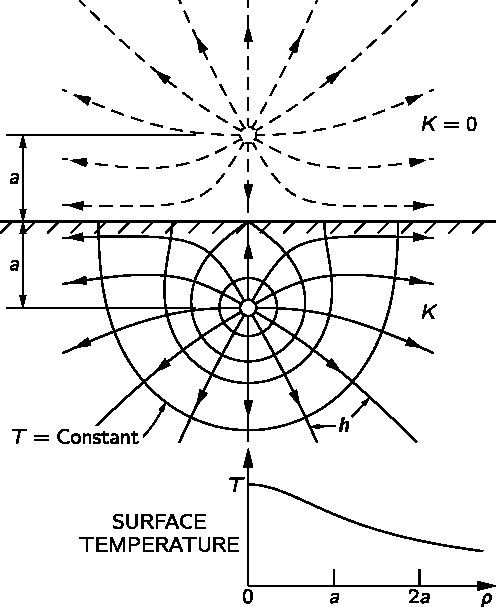
\includegraphics[width=1\linewidth]{fyz_fig725.pdf}
      \caption{Proudéní tepla a izotermy v blízkosti bodového zdroje tepla ve vzdálenosti \(a\) pod
        povrchem dobrého vodiče tepla. Myšlený zrcadlový zdroj se nachází mimo těleso.
        (\cite[s.~210]{Feynman02})}
      \label{fyz:fig725}
    \end{figure}

    Jak tedy najdeme elektrické pole, jež nemá složku kolmou na povrch, tj. takové, které je na
    povrchu vždy \emph{tangenciální}? Uvědomme si, že máme opačnou úlohu, než je ta o bodovém náboji
    v blízkosti rovinného vodiče. Tam jsme hledali pole \emph{kolmé} na povrch, neboť celý vodič měl
    stejný potenciál. V elektrické úloze jsme našli řešení pomocí zrcadlového obrazu bodového náboje
    za vodivou rovinou. Tutéž myšlenku můžeme použít opět. Budeme se snažit vybrat takový
    \uv{zrcadlový zdroj}, který automaticky vynuluje normálovou složku pole na povrchu.

    Řešení ukazuje obr. \ref{fyz:fig725}. Zrcadlový zdroj se \emph{stejným znaménkem} s toutéž
    velikostí, umístěný ve vzdálenosti \(a\) nad povrchem způsobí, že pole na povrchu bude vždy
    horizontální. Jeho normálové složky od obou zdrojů se vyruší.

    Tím je naše úloha o proudění tepla vyřešena. Z přímé analogie vyplývá, že teplota je všude tatáž
    jako potenciál dvou stejných bodových nábojů. Teplota \(T\) ve vzdálenosti \(r\) od izolovaného
    bodového zdroje \(G\) v nekonečném prostředí je
    \begin{equation}\label{fyz:eq769}
      T = \dfrac{G}{4\pi\lambda r}.
    \end{equation}
    (To je, samozřejmě, úplná analogie s výrazem \(\varphi = \frac{q}{4\pi\varepsilon_0r}\).)
    Teplotu v případě bodového zdroje spolu s jeho zrcadlovým zdrojem vyjadřuje výraz 
    \begin{equation}\label{fyz:eq770}
      T = \dfrac{G}{4\pi\lambda r_1} + \dfrac{G}{4\pi\lambda r_2}.
    \end{equation}
    Tento vzorec nám dává teplotu v celém tělese. Několik izotermických ploch je znázorněno na obr.
    \ref{fyz:fig725}. Ukázány jsou také křivky vektoru \(\vec{h}\), které lze dostat ze vztahu
    \(\vec{h} = -\lambda\nabla T\).
    
    Původně jsme se ptali na rozdělení teploty na povrchu. Pro bod na povrchu ve vzdálenosti
    \(\varrho\) od osy platí \(r_1= r_2 = \sqrt{\varrho^2 + a^2}\), takže
    \begin{equation}\label{fyz:eq771}
      T_{\text{na povrchu}} = \dfrac{1}{4\pi\lambda}\dfrac{2G}{\sqrt{\varrho^2 + a^2}}.
    \end{equation}
    Tato funkce je na obrázku také zakreslena. Teplota je, přirozeně, vyšší přímo nad zdrojem než 
    ve větší vzdálenosti. Je to úloha, kterou často potřebují řešit geofyzici. Teď vidíme, že jde o
    stejné problémy, jaké jsme řešili už v elektřině.

  \section{Napnutá membrána}\label{fyz:IIchapXIIsecIII}
    Nyní přejdeme ke zcela odlišné fyzikální situaci, která však vede k týmž rovnicím. Mějme ten­kou
    gumovou blánu, membránu, která byla natažena na velký vodorovný rám (jako kůže na bub­nu). Dále
    předpokládejme, že membrána je v jednom místě vysunuta nahoru a na jiném místě přitlačena dolů
    (obr. \ref{fyz:fig726}). Dokážeme popsat tvar její plochy? Ukážeme, jak lze tuto úlohu řešit
    když výchylky membrány nejsou příliš velké.

    \begin{figure}[ht!] %\ref{fyz:fig726}
      \centering
      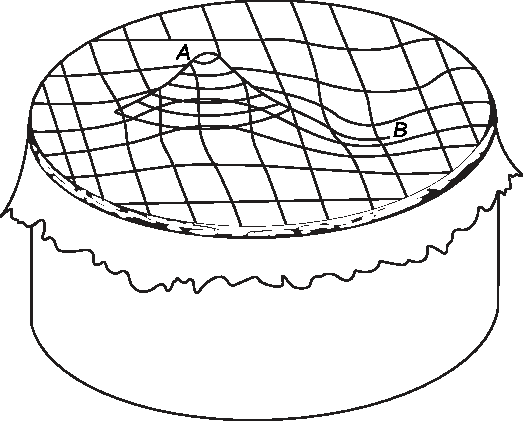
\includegraphics[width=1\linewidth]{fyz_fig726.pdf}
      \caption{Tenká gumová blána na válcovém rámu (jako kůže na bubnu). Jaký má tvar, je-li v bodě
        \(A\) vysunuta nahoru a v bodě \(B\) stlačena dolů? (\cite[s.~211]{Feynman02})}
      \label{fyz:fig726}
    \end{figure}

    V bláně působí síly, neboť je napnuta. Kdybychom kdekoliv v ní udělali malý řez, obě strany 
    řezu se od sebe oddálí (obr. \ref{fyz:fig727}).

    V bláně tedy existuje povrchové napětí, analogické s jednorozměrným napětím napjaté struny.
    Velikost povrchového napětí \(\tau\) definujeme jako sílu připadající na jednotkovou délku,
    která udržuje pohromadě strany takového řezu, jako je jeden z těch na obr. \ref{fyz:fig727}.

    \begin{figure}[ht!] %\ref{fyz:fig727}
      \centering
      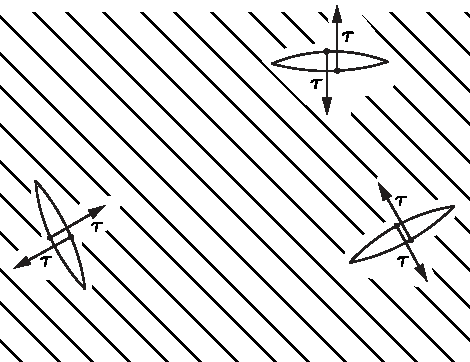
\includegraphics[width=0.9\linewidth]{fyz_fig727.pdf}
      \caption{Povrchové napětí \(\tau\) napnuté gumové blány je rovno síle připadající na jednotku
        délky a směřující kolmo na tuto délku (\cite[s.~211]{Feynman02})}
      \label{fyz:fig727}
    \end{figure}

    Nyní předpokládejme, že se díváme na vertikální řez membránou. Bude se jevit jako křivka podobná
    té, kteráje na obr. \ref{fyz:fig728}. Nechť \(u\) je vertikální výchylka membrány z její
    normální polohy a \(x\), \(y\) jsou souřadnice v horizontální rovině. (Zobrazený řez je
    rovnoběžný s osou \(x\).)

    Uvažujme malou část plochy membrány s délkou \(\Delta x\) šířkou \(\Delta y\). Na tuto plošku
    budou působit síly povrchového napětí, a to na každou její stranu. Síla na stranu \(1\) (viz
    obrázek) bude \(\tau_1\Delta y\) a bude směřovat tangenciálně vzhledem k ploše, tj. pod úhlem
    \(\Theta_1\) vzhledem k vodorovné rovině.

    Na stranu 2 bude působit síla \(\tau_2\Delta y\)  směřující pod úhlem \(\Theta_2\). (Podobné
    síly budou působit na druhých dvou stranách plošky, ale na chvíli na ně zapomeneme.) Výsledná
    síla, působící na plošku od stran \(1\) a \(2\) a směřující \emph{nahoru}, bude
    \begin{equation*}
      F = \tau_2\Delta y \sin\Theta_2 - \tau_1\Delta y \sin\Theta_1.
    \end{equation*}

    \begin{figure}[ht!] %\ref{fyz:fig728}
      \centering
      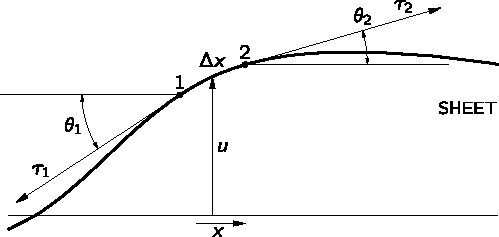
\includegraphics[width=1\linewidth]{fyz_fig728.pdf}
      \caption{Průřez vychýlenou blanou (\cite[s.~707]{Feynman02})}
      \label{fyz:fig728}
    \end{figure}

    Naše úvahy omezíme na malé deformace membrány, tj. na \emph{malé sklony}. Pak můžeme
    \(\sin\Theta\) nahradit funkcí \(\tan\Theta\), kterou lze psát jako \(\pder{u}{x}\). Síla
    potom je
    \begin{equation*}
      \Delta F = \left[
          \tau_2\left(\pder{u}{x}\right)_2 - 
          \tau_1\left(\pder{u}{x}\right)_1
        \right]\Delta y.
    \end{equation*}
    Veličinu v závorkách můžeme stejně dobře napsat (pro malá \(\Delta x\)) i ve tvaru
    \begin{equation*}
      \pder{}{x}\left(\tau\pder{u}{x}\right)\Delta x.
    \end{equation*}
    Pak bude platit
    \begin{equation*}
      \Delta F = \pder{}{x}\left(\tau\pder{u}{x}\right)\Delta x\Delta y.
    \end{equation*}
    Další příspěvek k \(\Delta F\) bude od sil působících na druhých dvou stranách plošky; výsledek
    je zřejmě
    \begin{equation}\label{fyz:eq772}
      \Delta F = \left[
          \pder{}{x}\left(\tau\pder{u}{x}\right) + 
          \pder{}{y}\left(\tau\pder{u}{y}\right)
        \right]\Delta x\Delta y.
    \end{equation}

    Deformace membrány vyvolávají vnější síly. Nechť \(f\) představuje sílu, která \emph{směřuje
    nahoru}, připadá na \emph{jednotku plochy} a působí na blánu (nějaký druh \uv{tlaku})
    \emph{následkem vnějších sil}. Když je membrána v rovnováze (statický případ), musí být tato
    síla vyvážena vnitřní silou, kterou jsme právě vypočetli (vztah \ref{fyz:eq772}), tj.
    \begin{equation*}
      f = -\dfrac{\Delta F}{\Delta x\Delta y}.
    \end{equation*}
    Vztah (\ref{fyz:eq772}) pak můžeme psát ve tvaru
    \begin{equation}\label{fyz:eq773}
      f = -\nabla\cdot(\tau\nabla u),
    \end{equation}   
    kde pod \(\nabla\) nyní samozřejmé rozumíme, operátor dvojrozměrného gradientu (\(\pder{}{x}\),
    \(\pder{}{y}\)). Máme tedy diferenciální rovnici, která uvádí do vztahu \(u(x, y)\) s vnějšími
    silami \(f(x, y)\) a s povrchovým napětím \(\tau(x, y)\), které se obecně mohou měnit na bláně
    od místa k místu. (Podobné rovnice popisují i deformace trojrozměrného pružného tělesa, ale my
    zůstaneme u dvou rozměrů.) Budeme se zajímat pouze o případ, kdy napětí \(\tau\) je po celé
    bláně konstantní. Pak můžeme místo rovnice (\ref{fyz:eq773}) napsat
    \begin{equation}\label{fyz:eq774}
      \nabla^2u = -\dfrac{f}{\tau},
    \end{equation}   

    Dostali jsme další rovnici, která je stejná jako v elektrostatice, tentokrát se však omezuje na
    dva rozměry. Výchylka \(u\) odpovídá potenciálu \(\varphi\) a \(f/\tau\) odpovídá
    \(\varrho/\varepsilon_0\). Proto všechny výsledky, které jsme získali pro nekonečné nabité
    roviny, dlouhé rovnoběžné dráty nebo nabité válce, lze přímo použít na napnutou membránu.

    \begin{figure}[ht!] %\ref{fyz:fig729}
      \centering
      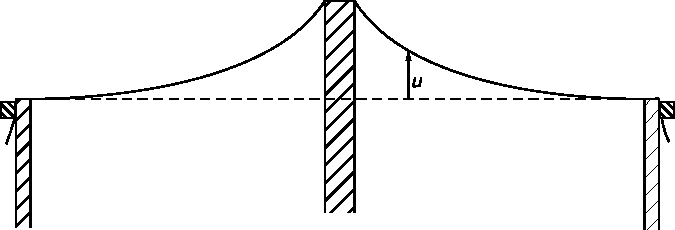
\includegraphics[width=0.9\linewidth]{fyz_fig729.pdf}
      \caption{Průřez napnutou gumovou fólií vysunutou nahoru pomocí okrouhlé tyče. Funkce \(u(x,
        y)\) je stejná jako elektrostatický potenciál \(\varphi(x, y)\) v blízkosti velmi dlouhé
        nabité tyče. (\cite[s.~213]{Feynman02})}
      \label{fyz:fig729}
    \end{figure}

    Předpokládejme, že v některých bodech vytáhneme membránu do určité \emph{výšky}, tj. na
    některých místech fixujeme hodnotu \(u\). To je analogie s elektrickou situací, ve které je na
    příslušných místech předepsaný potenciál. Tak například můžeme vyrobit kladný \uv{potenciál},
    tlačíme-li membránu předmětem, který má průřez tvaru příslušného válcového vodiče. Tlačíme-li na
    blánu, řekněme, okrouhlou tyčí, její povrch nabude takového tvaru, jaký ukazuje obr.
    \ref{fyz:fig729}. Výška \(u\) je stejná jako elektrostatický potenciál \(\varphi\) nabité
    válcové tyče. Klesá jako \(\ln(l/r)\). (\emph{Sklon} který odpovídá elektrickému poli \(E\),
    klesá jako \(1/r\).)

    Napnutá gumová blána se často používá jako způsob experimentálního řešení elektrických úloh.
    Analogie se tedy využívá v zpětném směru. Různými tyčemi a pruty se membrány vysouvají do výšek,
    které odpovídají potenciálům soustavy elektrod. Měřením výšky se pak zjišťuje elektrický
    potenciál v daných elektrických podmínkách. Analogie se provádí ještě dále. Umístí-li se na
    membránu malé kuličky, jejich pohyb odpovídá přibližně pohybu elektronů v příslušném elektrickém
    poli. Tak je opravdu možné pozorovat, jak se \uv{elektrony} pohybují po svých trajektoriích.
    Tato metoda se využívala při projektování složité geometrie mnohých fotonásobičů (takových, jako
    ty, které se používají v scintilačních počítačích. Dnes se samozřejmě určují pole numerickými
    metodami.

  \twocolumn[\section{Difúze elektronů. Kulově symetrický zdroj v homogenním
  prostředí}\label{fyz:IIchapXIIsecIV}] 
  
    Uvedeme další příklad, který vede k rovnici téhož druhu, týkající se tentokrát difúze. V
    ka­pitole \ref{fyz:IchapXLIII} dílu \ref{part:FYZI} jsme se zabývali difuzí jednoho plynu v
    druhém. Tentokrát vezmeme jiný příklad - difúzi neutronů v takové látce jako grafit. Mluvit o
    grafitu (čistá forma uhlíku) jsme se rozhodli proto, že uhlík nepohlcuje pomalé neutrony.
    Neutrony v něm putují volně. Předtím, než jsou jádrem rozptýleny a vychýleny do nového směru,
    projdou v přímém směru průměrně několik centimetrů. Proto máme-li velký grafitový blok s hranou
    dlouhou mnoho metrů, budou neutrony nacházející se původně v jednom místě v něm difundovat do
    jiných míst. Je nutné popsat jejich střední chování, tj. jejich \textbf{střední tok}.

    Nechť \(N(x, y, z)\Delta V\) je počet neutronů v elementu objemu \(\Delta V\) se středem v bodě
    \((x, y, z)\). V důsledku svého pohybu opustí některé z neutronů \(\Delta V\) a jiné do něj
    přibudou. Je-li v jedné oblasti víc neutronů než v sousední, odejde víc neutronů z první do
    druhé, nežli přijde zpět; vznikne výsledný tok neutronů. Na základě stejných úvah jako v
    kapitole \ref{fyz:IchapXLIII} popíšeme tok pomocí vektoru hustoty toku \(\vec{J}\). Jeho
    \(x\)-ová složka představuje výsledný počet neutronů procháze­jících za jednotku času
    jednotkovou plochou kolmou na směr osy \(x\). Zjistili jsme, že
    \begin{equation*}
      J_x = -D\diffp{N}{x},
    \end{equation*} 
    kde koeficient difúze \(D\) je určen střední rychlostí \(v\) a střední volnou dráhou \(l\) mezi
    srážkami neutronů způsobujícími jejich rozptyl
    \begin{equation*}
      D = \frac{1}{3}lv.
    \end{equation*}
    Vektorová rovnice určující \(\vec{J}\) je
    \begin{equation}\label{fyz:eq775}
      \vec{J} = -D\nabla\vec{N},
    \end{equation} 

    Počet neutronů, které projdou za jednotku času nějakým plošným elementem \(\dd{S}\), je roven
    \(\vec{J}\cdot\vec{n}\dd{S}\), kde, jako obvykle, \(\vec{n}\) je jednotkový vektor ve směru
    normály k plošnému elementu. Výsledný tok z \emph{objemového elementu} pak (na základě obvyklých
    gaussovských úvah) bude \(\nabla\cdot\vec{J}\dd{V}\). Tento tok by způsobil pokles počtu
    neutronů v elementu \(\Delta V\) v čase, pokud by se však v \(\Delta V\) další neutrony
    nevytvářely (nějakým jademým procesem). Nacházejí-li se v uvažovaném objemu zdroje, generující v
    jednotce objemu \(s\) neutronů za jednotku času, výsledný tok z \(\Delta V\) bude roven \((s -
    \diffp{N}{t})\Delta V\). Pak dostaneme
    \begin{equation}\label{fyz:eq776}
      \nabla\cdot\vec{J}= s - \diffp{N}{t},
    \end{equation} 
    Když do (\ref{fyz:eq776}) dosadíme \(\vec{J}\) podle (\ref{fyz:eq775}), dostaneme \emph{rovnici
    difúze neutronů}
    \begin{equation}\label{fyz:eq777}
      \nabla\cdot(-D\nabla\vec{N})= s - \diffp{N}{t},
    \end{equation} 

    Ve statickém případě, kdy \(\diffp{N}{t} = 0\), dostáváme opět rovnici (\ref{fyz:eq759}). To, co
    víme z elektrostati­ky, můžeme využít i k řešení úloh o difúzi neutronů. Řešme tedy nějakou
    úlohu. (Třeba se podivíme: \uv{Proč řešit další úlohu, když už jsme všechny vyřešili v
    elektrostatice?} Tentokrát ji však můžeme vyřešit rychleji, neboť už \emph{máme} elektrostatické
    úlohy vyřešeny.)

    \begin{figure}[ht!]
      \centering
      \subcaptionbox{\label{fyz:fig730a}}{\luafigure[0.6]{fyz_fig730a.pdf}}               \newline
      \subcaptionbox{\label{fyz:fig730b}}{\luafigure[0.6]{fyz_fig730b.pdf}}
      \label{fyz:fig730}
      \caption{a) Neutrony vznikají homogenně v kouli s poloměrem a uvnitř velkého grafitového bloku
        a difundují ven. Ukazuje se, že hustota neutronů \(N\) je funkcí vzdáleností \(r\) od středu
        zdroje, b) Analogická elektrostatická situace: homogenně nabitá koule, přičemž \(N\)
        odpovídá \(\varphi\) a \(\vec{J}\) odpovídá \(\vec{E}\) (\cite[s.~215]{Feynman02})}
    \end{figure}

    Předpokládejme, že máme blok materiálu, v němž se, řekněme, štěpením uranu, homogenně generují
    neutrony v kulové oblasti s poloměrem \(a\) (obr. \ref{fyz:fig730a}) Chtěli bychom vědět: Jaká
    je hustota neutronů kdekoliv v prostoru? Nakolik homogenní je jejich hustota v oblasti, kde se
    generují? V jakém poměřu je hustota neutronů ve středu k hustotě neutronů na povrchu oblasti
    jejich zdroje? Odpovědi na tyto otázky se najdou snadno. Hustota zdroje s nahrazuje hustotu
    \(\varrho\), takže naše úloha je totožná s úlohou o homogenně nabité kouli. Najít \(N\) je
    totéž, jako najít potenciál \(\varphi\). Pole uvnitř, jakož i vně, homogenně nabité koule už
    jsme našli. Můžeme je integrovat, aby­chom dostali potenciál. Vně koule je potenciál roven
    \(\frac{Q}{4\pi\varepsilon_0r}\) kde celkový náboj \(Q\) je dán výrazem \(\frac{4\pi
    a^3\varrho}{3}\). Tedy
    \begin{equation}\label{fyz:eq778}
      \varphi_{\text{vně}} = \dfrac{\varrho a^3}{3\varepsilon_0r}.
    \end{equation}
    Ve vnitřních bodech je pole vytvářeno pouze nábojem \(Q(r)\) uvnitř koule o poloměru \(r\), tj.
    \(Q(r)=4πr^3ρ/3\), takže 
    \begin{equation}\label{fyz:eq782}
      E=\dfrac{ρr^3}{ϵ_0}.
    \end{equation}
    Intenzita pole roste lineárně s \(r\). Integrováním \(E\) dostaneme
    \begin{equation*}
      ϕ_{\text{uvnitř}}=−\dfrac{ρr^2}{6ϵ_0} + \text{ konst}.
    \end{equation*}
    Při poloměru \(a\) musí být \(ϕ_{\text{uvnitř}}\) stejné jako \(ϕ_{\text{vně}}\), takže
    konstanta musí být rovna \(ρa^2/2ϵ^0\). (Předpokládejme, že ve velkých vzdálenostech od zdroje
    je \(\varphi\) rovno nule, což pro neutrony bude odpovídat nulovému \(N\).) Proto
    \begin{equation}\label{fyz:eq788}
      ϕ_{\text{uvnitř}}=\dfrac{ρ^3}{ϵ_0}\left(\dfrac{3a^2}{2}−\dfrac{r^2}{2}\right).
    \end{equation}
    Hustotu neutronů se v naší úloze dovíme ihned. Výsledek je
    \begin{align}
      N_\text{vně}   &=\dfrac{Sa^3}{3Dr},                                        \label{fyz:eq789}\\
      \shortintertext{a}
      N_\text{uvnitř}&=\dfrac{S}{3D}\left(\dfrac{3a^2}{2}−\dfrac{r^2}{2})\right).\label{fyz:eq790} 
    \end{align}
    Graf \(N\) jako funkce \(r\) je na obr. \ref{fyz:fig730a}.

    Jaký je nyní poměr hustoty ve středu k hustotě na okraji? Ve středu (\(r = 0\)) je hustota přímo
    úměrná veličině \(3a^2/2\). Na kraji (\(r= a\)) je přímo úměrná veličině \(2a^2/2\), tj. poměr
    obou hustot je roven \(3/2\). Homogenní zdroj tedy negeneruje homogenní hustotu neutronů. Jak
    vidíte, naše vědomosti z elektrostatiky nám umožňují dobrý start do fyziky jaderných reaktorů.

    Fyzikálních situací, v nichž difúze hraje velkou úlohu, je mnoho. I pohyb iontů v kapalině nebo
    elektronů v polovodiči probíhá podle téže rovnice. Znovu a znovu docházíme ke stejným rovnicím.

  \section{Bezvírové proudění kapaliny. Obtékání koule}\label{fyz:IIchapXIIsecV} Nyní vezměme
  příklad, který ve skutečnosti není příliš dobrý, neboť rovnice, které přitom použijeme, nebudou
  uvažovaný jev popisovat zcela obecně, ale pouze v umělé idealizované situaci. Uvažujme úlohu o
  \emph{proudění vody}. V případě napnuté membrány představovaly naše rovnice aproximaci platící
  pouze pro \emph{malé výchylky}. Při zkoumání proudění vody takovou aproximaci nebudeme provádět;
  musíme udělat taková omezení, která se k proudění reálné vody vůbec nehodí. Budeme se totiž
  zabývat pouze případem ustáleného proudění \textbf{nestlačitelné}, \textbf {neviskózní} a \textbf
  {nevírové} kapaliny. Proudění pak budeme charakterizovat udáním rychlosti \(v(r)\) jako funkce
  polohy \(r\). Je-li ustálené (jediný případ pro který existuje elektrostatická analogie), nezávisí
  \(v\) na čase. Je-li \(ρ\) hustota kapaliny, pak \(ρv\) znamená hmotnost, jež prochází jednotkovou
  plochou za jednotku času. Podle principu zachování látky bude divergence vektoru \(ρv\) obecně
  rovna změně hmotnosti látky v jednotkovém objemu za jednotku času. Budeme předpokládat, že
  nedochází k procesům nepřetržitého vznikání nebo zanikání hmotnosti. Princip zachování látky pak
  požaduje, aby \(∇\cdot ρ\vec{v}=0\). (Obecně by na pravé straně této rovnice mělo být \(-\diffp
  ρt\), ale \(ρ\) se měnit nemůže, neboť naše kapalina je nestlačitelná.) Protože \(ρ\) je všude
  stejné, můžeme jím krátit a naše rovnice má jednoduchý tvar:
  \begin{equation*}
    ∇\cdot\vec{v}=0.
  \end{equation*}
  Výborně! Opět dostáváme elektrostatiku (bez nábojů); je to právě taková rovnice jako
  \(∇⋅\vec{E}=0\). Ale není to tak jednoduché. Elektrostatika nevyplývá jen z toho, že
  \(∇⋅\vec{E}=0\). Zakládá se na páru rovnic. Jedna rovnice nám mnoho nepoví; potřebujeme ještě
  doplňující rovnici. Aby byla shoda s elektrostatikou, mělo by také platit, že rotace vektoru
  \(\vec{v}\) je rovna nule. Ale pro reálné kapaliny to obecně neplatí. Ve většině kapalin obvykle
  nějaké víření vzniká, musíme se tedy omezit na situace, V nichž víření kapaliny nenastává. Takové
  proudění se často nazývá bezvírová. Tak či onak, přijmeme-li všechny naše předpoklady, dokážeme si
  představit takový případ proudění kapaliny, který je analogický s elektrostatikou. Požadujeme
  tedy, aby
  \begin{subequations} \label{fyz:eq791}
    \begin{align}
      ∇⋅\vec{v}     &=0      \label{fyz:eq791a} \\
      \shortintertext{a}
      ∇\times\vec{v}&=0      \label{fyz:eq791b}
    \end{align}
  \end{subequations}

    \begin{figure}[ht!] %\ref{fyz:fig731}
      \centering
      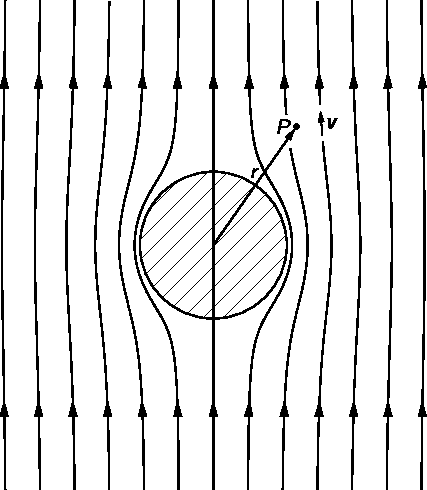
\includegraphics[width=0.7\linewidth]{fyz_fig731.pdf}
      \caption{Pole rychlosti při bezvírovém obtékání koule kapalinou
              (\cite[s.~217]{Feynman02})}
      \label{fyz:fig731}
    \end{figure}

    Chceme zdůraznit, že i když ty případy, v nichž proudění kapaliny probíhá podle těchto rovnic,
    nepředstavují ani zdaleka většinu možných případů, několik jich přece existuje. Musí to být
    takové případy, kdy můžeme zanedbat povrchové napětí, stlačitelnost a viskozitu a kdy můžeme
    dále předpokládat, že proudění je bezvírové. Pro reálnou vodu platí tyto předpoklady tak zřídka,
    že matematik John von Neumann řekl, že lidé, kteří analyzují rovnice (\ref{fyz:eq791a}) a
    (\ref{fyz:eq791b}), zkoumají \uv{suchou vodu}. (Problémem proudění kapaliny se budeme podrobněji
    zabývat v kapitolách \ref{fyz:IIchapXL} a \ref{fyz:IIchapXLI}.)
    
    Protože \(\nabla\times\vec{v} = 0\), rychlost „suché vody“ lze zapsat jako gradient nějakého
    potenciálu: 
    \begin{equation}\label{fyz:eq792}
      \vec{v}=−∇ψ.
    \end{equation}

    Jaký fyzikální význam má \(ψ\). Žádný zvláštní. Rychlost lze napsat jako gradient potenciálu
    prostě proto, že proudění je bezvírové. \(ψ\) se nazývá \textbf{potenciál rychlosti} pouze na
    základě analogie s elektrostatikou, ale s potenciální energií nesouvisí takovým způsobem jako
    \(\varphi\). Protože divergence vektoru \(\vec{v}\) je rovna nule, dostáváme 
    \begin{equation}\label{fyz:eq793}
      ∇⋅(∇ψ)=∇^2ψ=0.
    \end{equation}
    Potenciál rychlosti \(ψ\) vyhovuje téže diferenciální rovnici jako elektrostatický potenciál
    v prázdném prostoru (tj. tam, kde \(ρ=0\)). 

    Vezměme nějakou úlohu o bezvírovém proudění a přesvědčíme se, zda ji dokážeme řešit metodami,
    které jsme se naučili. Uvažujme kouli padající v kapalině. Bude-li se pohybovat příliš pomalu,
    budou důležité síly vnitřního tření, které zanedbáváme. Bude-li se pohybovat příliš rychle, v
    její stopě se objeví malé víry (turbulence) a bude docházet k určitému víření vody. Ale
    nepohybuje-li se koule příliš rychle, ani příliš pomalu, proudění vody bude více méně vyhovovat
    našim předpokladům a pohyb vody můžeme popsat našimi jednoduchými rovnicemi.
    
    Co se děje, je vhodné popisovat ve vztažné soustavě \emph{spojené s koulí}. V této vztažné
    soustavě si položme otázku: jak voda proudí okolo nepohyblivé koule, když proudění ve velkých
    vzdálenostech je homogenní, tj. když daleko od koule je tok všude stejný? Charakter proudění v
    blízkosti koule je znázorněn na obr. \ref{fyz:fig731} pomocí proudnic. Tyto křivky, které jsou
    vždy rovnoběžné s \vec{v}, odpovídají siločárám elektrického pole. Chceme dostat kvantitativní
    popis pole rychlosti, tj. výraz pro rychlost v libovolném bodě \(P\).

    Rychlost můžeme dostat z gradientu \(ψ\) proto nejprve vypočítejme potenciál. Chceme najít
    potenciál, který všude splňuje rovnici (\ref {fyz:eq793}) a kromě toho vyhovuje dvěma omezením:
    \begin{enumerate}
      \item  ve vnitřní oblasti ohraničené povrchem naší koule není proudění,
      \item  ve velkých vzdálenostech je proudění konstantní.
    \end{enumerate}
    Aby bylo vyhověno podmínce 1, musí být složka \(\vec{v}\) kolmá na povrch koule, rovna nule. To
    znamená, že \(\diffp ψt\)je rovno nule při \(r = a\). Aby se vyhovělo podmínce 2, musí platit,
    že \(\diffp ψt = v_0\) se všech bodech, pro které \(r≫a\). Přesně vzato, elektrostatický případ,
    který odpovídá naší úloze, neexistuje. Naše úloha ve skutečnosti odpovídá umístění koule s
    \emph{nulovou} permitivitou do homogenního elektrického pole. Kdybychom znali řešení úlohy o
    kouli s relativní permitivitou \(\varepsilon_r\) umístěné v homogenního poli, pak bychom
    položením \(\varepsilon_r = 0\) ihned dostali řešení naší úlohy. 
    
    Tuto konkrétní elektrostatickou úlohu jsme dosud vlastně podrobněji nepočítali. Udělejme to však
    nyní. (Mohli bychom přímo řešit úlohu o toku s \(\vec{v}\) a \(ψ\) ale budeme používat
    \(\vec{E}\) a \(\varphi\) neboť jsme na ně zvyklí.)

    Úloha vyžaduje najít takové řešení rovnice \( ∇^2ϕ=0\), aby pro velké hodnoty \(r\) byla řešením
    rovnice \(E=−∇ϕ\) konstanta, řekněme \(E_0\),a aby při \(r=a\) byla radiální složka vektoru
    \(\vec{E}\) rovna nule, tj. aby platilo



  \section{Osvětlení. Homogenní osvětlení roviny}\label{fyz:IIchapXIIsecVI}

    \begin{figure}[ht!] %\ref{fyz:fig732}
      \centering
      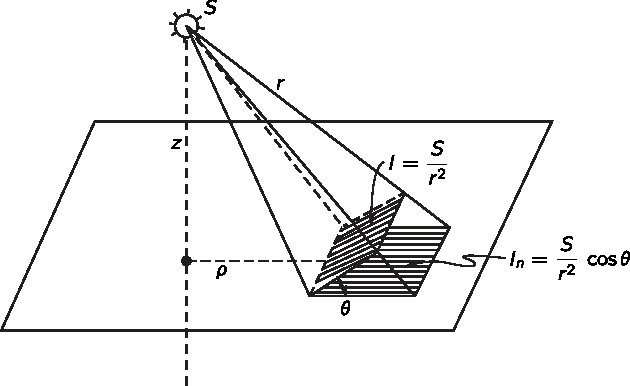
\includegraphics[width=1\linewidth]{fyz_fig732.pdf}
      \caption{Osvětlení \(E_n\) plochy je rovno světelnému toku dopadajícímu (za jednotku času) na
        plošnou jednotku této plochy. (\cite[s.~220]{Feynman02})}
      \label{fyz:fig732}
    \end{figure}

  \section{\uv{Fundamentální jednotka} přírody}\label{fyz:IIchapXIIsecVII}



  \section{Příklady a cvičení}\label{fyz:IIchapXIIsecVIII}














\todo[inline]{Kapitola fey2c12 je nedodělaná, obsahuje pouze obrázky}
%} %tikzset
%---------------------------------------------------------------------------------------------------
